\documentclass[border=6pt]{standalone}
\usepackage{tikz}
\usetikzlibrary{arrows.meta,positioning,fit,calc}
\definecolor{fg}{HTML}{3B3220}
\definecolor{fgbody}{HTML}{544736}
\definecolor{stroke}{HTML}{7A5A10}
\definecolor{surf}{HTML}{FAF6EE}
\definecolor{surfemph}{HTML}{F2E9D4}
\definecolor{surfact}{HTML}{F6E7E0}
\definecolor{bdim}{HTML}{CFC6B2}
\definecolor{bemph}{HTML}{7A5A10}
\definecolor{bact}{HTML}{8F1D1D}
\begin{document}
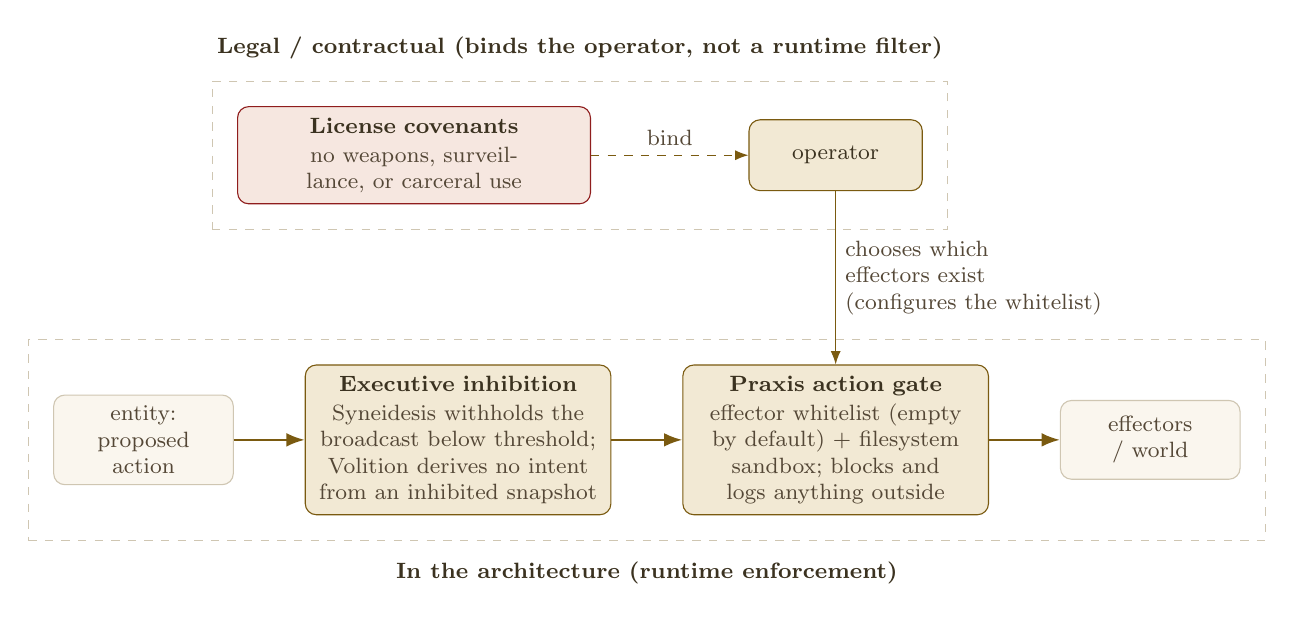
\begin{tikzpicture}[
  font=\small,>=Latex,
  io/.style={draw=bdim, rounded corners, fill=surf, text=fgbody, align=center, minimum height=10mm, text width=20mm, inner sep=4pt, font=\footnotesize},
  gate/.style={draw=bemph, rounded corners, fill=surfemph, text=fgbody, align=center, minimum height=15mm, text width=36mm, inner sep=4pt, font=\footnotesize},
  cov/.style={draw=bact, rounded corners, fill=surfact, text=fgbody, align=center, text width=42mm, inner sep=4pt, font=\footnotesize},
  op/.style={draw=bemph, rounded corners, fill=surfemph, text=fg, align=center, minimum height=9mm, minimum width=22mm, inner sep=4pt, font=\footnotesize},
]
% runtime flow row (bottom): entity -> inhibition -> praxis -> world
\node[io] (entity) {entity:\\proposed action};
\node[gate, right=9mm of entity] (inh) {\textcolor{fg}{\textbf{Executive inhibition}}\\[1pt]Syneidesis withholds the broadcast below threshold; Volition derives no intent from an inhibited snapshot};
\node[gate, right=9mm of inh] (praxis) {\textcolor{fg}{\textbf{Praxis action gate}}\\[1pt]effector whitelist (empty by default) $+$ filesystem sandbox; blocks and logs anything outside};
\node[io, right=9mm of praxis] (world) {effectors / world};
\draw[->, thick, draw=stroke] (entity) -- (inh);
\draw[->, thick, draw=stroke] (inh) -- (praxis);
\draw[->, thick, draw=stroke] (praxis) -- (world);
\node[draw=bdim, dashed, fit=(entity)(inh)(praxis)(world), inner sep=9pt] (regA) {};
\node[font=\footnotesize\bfseries, text=fg, below=1.5mm of regA] {In the architecture (runtime enforcement)};
% operator above praxis
\node[op, above=22mm of praxis] (op) {operator};
\draw[->, draw=stroke] (op) -- node[right, font=\footnotesize, align=left, text=fgbody]{chooses which\\effectors exist\\(configures the whitelist)} (praxis.north);
% covenants to the left of operator (top legal region)
\node[cov, left=20mm of op] (cov) {\textcolor{fg}{\textbf{License covenants}}\\[1pt]no weapons, surveillance, or carceral use};
\draw[->, dashed, draw=stroke] (cov) -- node[above, font=\footnotesize, text=fgbody]{bind} (op);
\node[draw=bdim, dashed, fit=(cov)(op), inner sep=9pt] (regB) {};
\node[font=\footnotesize\bfseries, text=fg, above=1.5mm of regB] {Legal / contractual (binds the operator, not a runtime filter)};
\end{tikzpicture}
\end{document}
